\documentclass[runningheads]{llncs}
\usepackage[T1]{fontenc}

\usepackage[table]{xcolor}

\usepackage{booktabs}
\usepackage[pdfstartview=XYZ,
bookmarks=true,
colorlinks=true,
linkcolor=blue,
urlcolor=blue,
citecolor=blue,
pdftex,
bookmarks=true,
linktocpage=true, % makes the page number as hyperlink in table of content
hyperindex=true
]{hyperref}

\usepackage{rotating} % Rotating table
\usepackage{subcaption}
\usepackage{graphicx}
\usepackage{multirow}
\usepackage{amsmath}
\usepackage{array} % necessary for word wrap within a table



\title{Buyer Beware: Understanding the trade-off between utility and risk in CART based models using simulation data}
\titlerunning{Buyer Beware}

\author{Jonathan Latner\inst{1}\orcidID{0000-0002-1825-0097} \and
Marcel Neunhoeffer\inst{1,2}\orcidID{0000-0002-9137-5785}  \and
J\"{o}rg Drechsler\inst{1,2,3}\orcidID{0009-0009-5790-3394}}

\authorrunning{Latner et al.}


\institute{Institute for Employment Research, Nuremberg, Germany 
\email{\{jonathan.latner, marcel.neunhoeffer,joerg.drechsler\}@iab.de} \and
Ludwig-Maximilians-Universit\"at, Munich, Germany \and
University of Maryland, College Park, USA
}



\begin{document}

\maketitle 

\begin{abstract}

This study examines the trade-off between utility and privacy when generating synthetic data using Classification and Regression Trees (CART) as a Synthetic Data Generator (SDG). Using low-dimensional simulated data with binary variables, we highlight the limitations of CART in mitigating disclosure risks, demonstrate how common privacy metrics do not capture these risks, and propose parameter modifications to balance the trade-off. Our findings underscore the challenges in identifying privacy risks and the necessity of sacrificing utility to enhance privacy, raising critical questions for synthetic data practices.

\keywords{Synthetic data \and Privacy \and CART \and synthpop}
\end{abstract}

\section{Introduction}

The generation of synthetic data has gained prominence as a means to share data while preserving privacy. It is well-established that there is a trade-off between utility and privacy in synthetic data generation \cite{duncan2004database}. CART models, a widely used synthetic data generator (SDG), are noted for their high utility and relatively low privacy risks compared to other methods \cite{little2022comparing,dankar2021fake}. However, the mechanisms that enable CART to minimize this trade-off remain underexplored.

In this paper, we evaluate whether CART-based SDGs effectively mitigate the risk-utility trade-off.  To do so, we borrow from Reiter et al., \cite{reiter2014bayesian} and simulate a low-dimensional data set with 1000 and four binary variables.  Crucially, the last or 1000$^th$ observation is a unique combination of the four binary variables.  In so doing, we create data with an observation we want to protect with synthetic data generated from a CART model.  

In this paper, we seek to make three main contributions.  First, we assess whether we are able to adequately capture the disclosure risks that exist in our simulated data.  Concerns about how to measure utility or privacy in synthetic data are well established.  The problem is not a lack of measures, but rather there is little agreement on which measures are correct for what type of data.  We use common utility and privacy metrics that are available in the Synthpop package \cite{nowok2016synthpop}.  While the results indicate that CART models generate synthetic data with both high levels of utility and privacy, we show that the synthetic data do not protect the disclosive record and this dislosure is not captured by common privacy metrics.  

Second, we explore parameter modifications to the CART-based synthesizer as a potential solution to balance privacy and utility.  On the one hand, we show that one can easily create synthetic data from a CART-based synthesizer that provides a high degree of protection.  On the other hand, we show that one must sacrifice the high levels of utility generated using the default parameters.  Therefore, CART-based synthesizers are capable of generating synthetic data with high levels of privacy protection, but users would have to choose to sacrifice utility even if there is no indication of a disclosure risk.

Third, we propose and evaluate a new implementation of a privacy metric originally developed by Reiter et al., \cite{reiter2014bayesian}. 

<Insert MN text>

In summary, we show that synthetic data from a CART-based SDG are more sensitive to the risk-utility trade-off than was understood from previous research.  Admittedly, we demonstrate this problem using a simulated data set that is unlikely to be used in the real world.  However, the bigger problem is that we demonstrate that a disclosure risk exists in synthetic data that are not captured by common privacy metrics.  If common privacy metrics cannot capture disclosure risks in synthetic data that we know exist (because we created them), then this reduces our confidence that these metrics can capture disclosure risks that we may not know exist.  While we propose solutions to this problem that operate with low-dimensional data, users interested in generating synthetic data should be aware of the challenges we describe here.

\section{Data and Methods}

Following Reiter et al. \cite{reiter2014bayesian}, we simulate one data set with 1.000 observations and four binary categorical variables.  This is our `original' data set.  The first 999 records were sampled from a multinomial distribution for all combinations of var1(0,1), var2(0,1), var3(0,1), var4(0,1), except the last 1000$^{th}$ record was a unique combination (var1 = 1, var2 = 1, var3 = 1, var4 = 1).  

Figure \ref{fig:frequency_compare} shows the frequency distribution within each of the four variables and figure \ref{fig:histogram_compare} the frequency histogram across all four variables.  They are not evenly distributed within or across the variables because the data are generated from one random sample.  If we were to create 100 samples, then the data would be more even within each of the variables (50\%) and across all four variables (66\%), with the exception of the 1,1,1,1 combination.  However, the critical point is that there is one observation with combination (1,1,1,1) that is not visible if we look at the distribution within each of the variables.

% \begin{figure}[!h]
%     \centering
%     \caption{Original data}
%     \begin{subfigure}{0.48\textwidth}
%         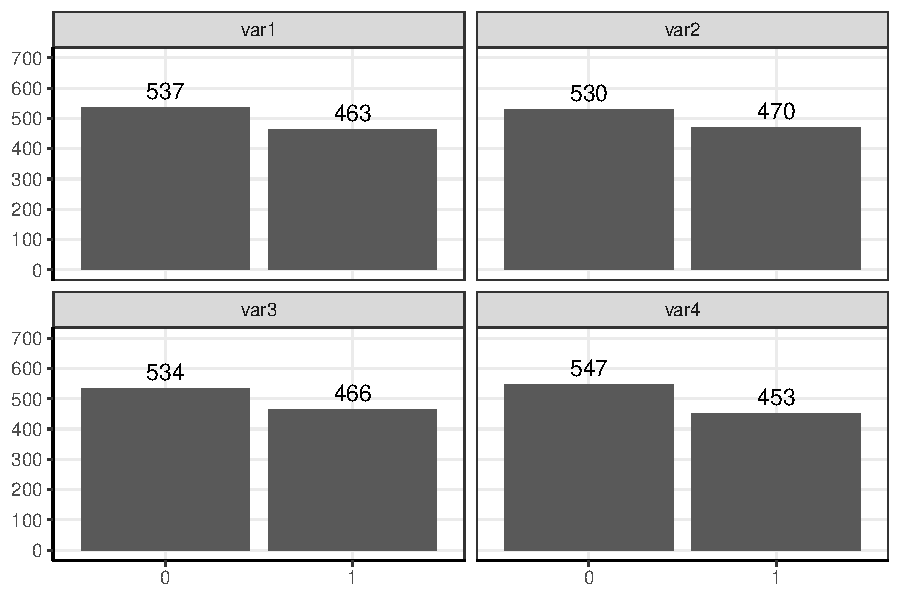
\includegraphics[width=\textwidth]{../graphs/graph_cart_frequency.pdf}
%         \caption{Frequency}
%         \label{fig:frequency}
%     \end{subfigure}
%     \hfill
%     \begin{subfigure}{0.48\textwidth}
%         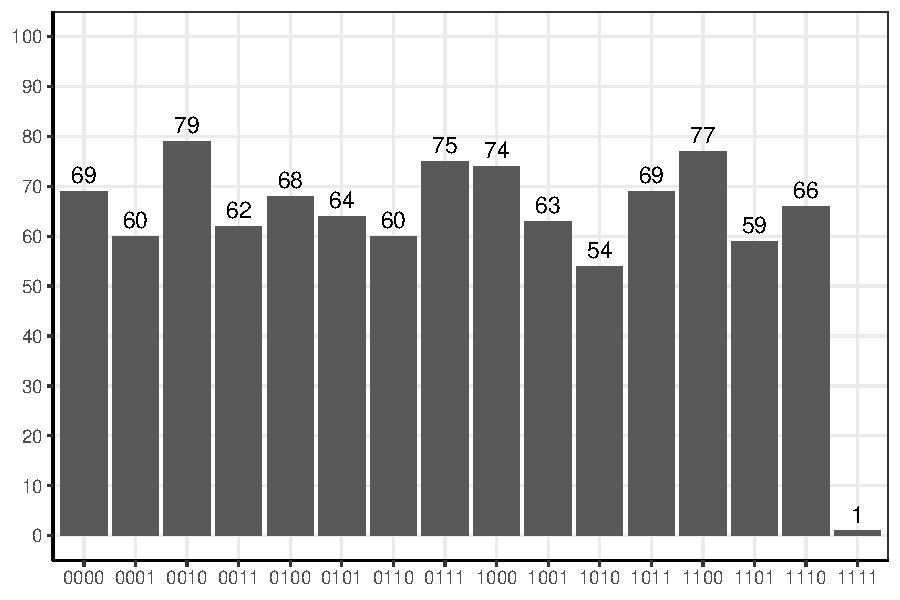
\includegraphics[width=\textwidth]{../graphs/graph_cart_histogram.pdf}
%         \caption{Histogram}
%         \label{fig:histogram}
%     \end{subfigure}
%     \label{fig:original}
% \end{figure}

Next, we generate one synthetic data from a CART-based SDG from the Synthpop package in R with default parameters (seed=1237).  Figure \ref{fig:frequency_compare} shows the frequency distribution within each of the four variables and figure \ref{fig:histogram_compare} the frequency histogram across all four variables.  Not only do the synthetic data capture the frequency of values within the four variables, but also across all four variables.  The good news is that this means that the synthetic data have high levels of utility.  The bad news is that the synthetic data perfectly replicates the single disclosive record.

\begin{figure}[!h]
    \centering
    \caption{Compare original and synthetic data}
    \begin{subfigure}{0.48\textwidth}
        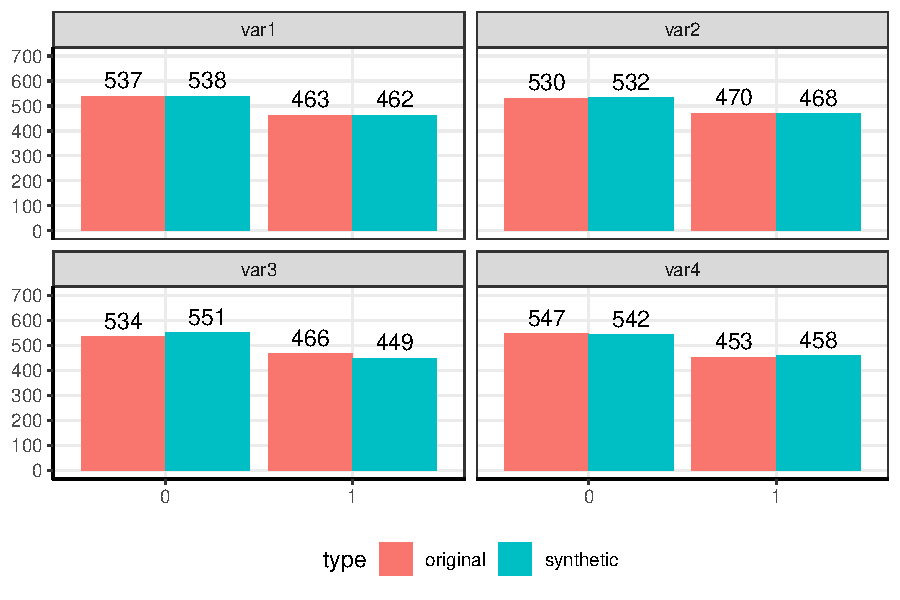
\includegraphics[width=\textwidth]{../graphs/graph_cart_frequency_compare.pdf}
        \caption{Frequency}
        \label{fig:frequency_compare}
    \end{subfigure}
    \hfill
    \begin{subfigure}{0.48\textwidth}
        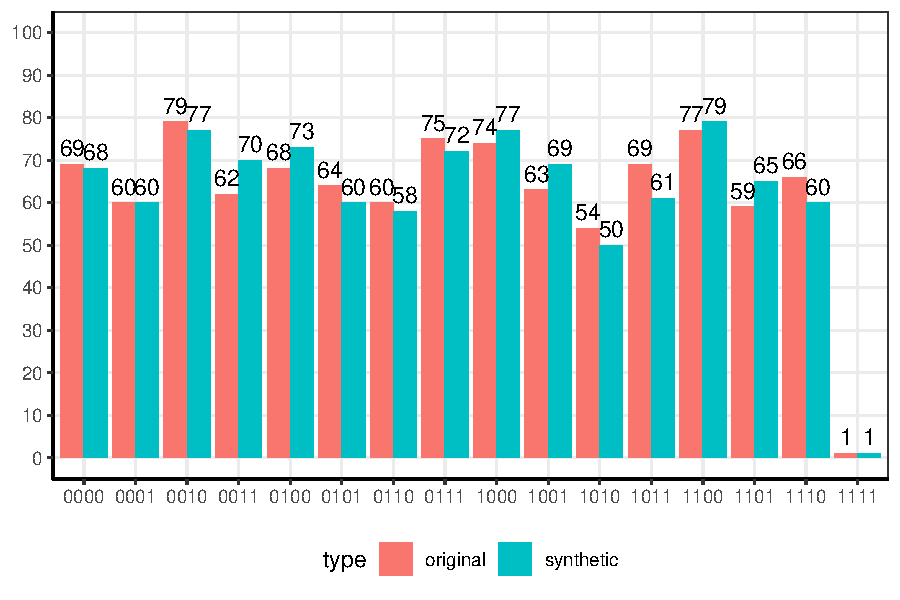
\includegraphics[width=\textwidth]{../graphs/graph_cart_histogram_compare.pdf}
        \caption{Histogram}
        \label{fig:histogram_compare}
    \end{subfigure}
    \label{fig:compare}
\end{figure}

As a sensitivity test, we create 10 synthetic data sets from the original data, as shown in figure \ref{fig:cart_histogram_compare_10} and table \ref{table:frequency_10_data_sets}.  Out of 10 synthetic data sets, the frequency of the disclosive record ranges from 0 (2 data sets), 1 (5 data sets), 2 (1 data sets), and 3 (2 data sets).\footnote{For reference, if we created 100 synthetic data sets the frequency of the disclosive record would be similar, ranging from 0 (41 data sets), 1 (38 data sets), 2 (14 data sets), and 3 (7 data sets).}  As a result, regardless of whether one, five, or ten synthetic data sets were released, it would be clear which record was the disclosive record.  As a result, synthetic data from CART models do not protect the unique observation in our simulated data set.  The reason is that in our data with binary categorical data, a record may not be in the synthetic data if it is in the original data, but it can only be in the synthetic data if it is also in the original data.  

\begin{figure}[!h]
    \centering
    \caption{Frequency}
    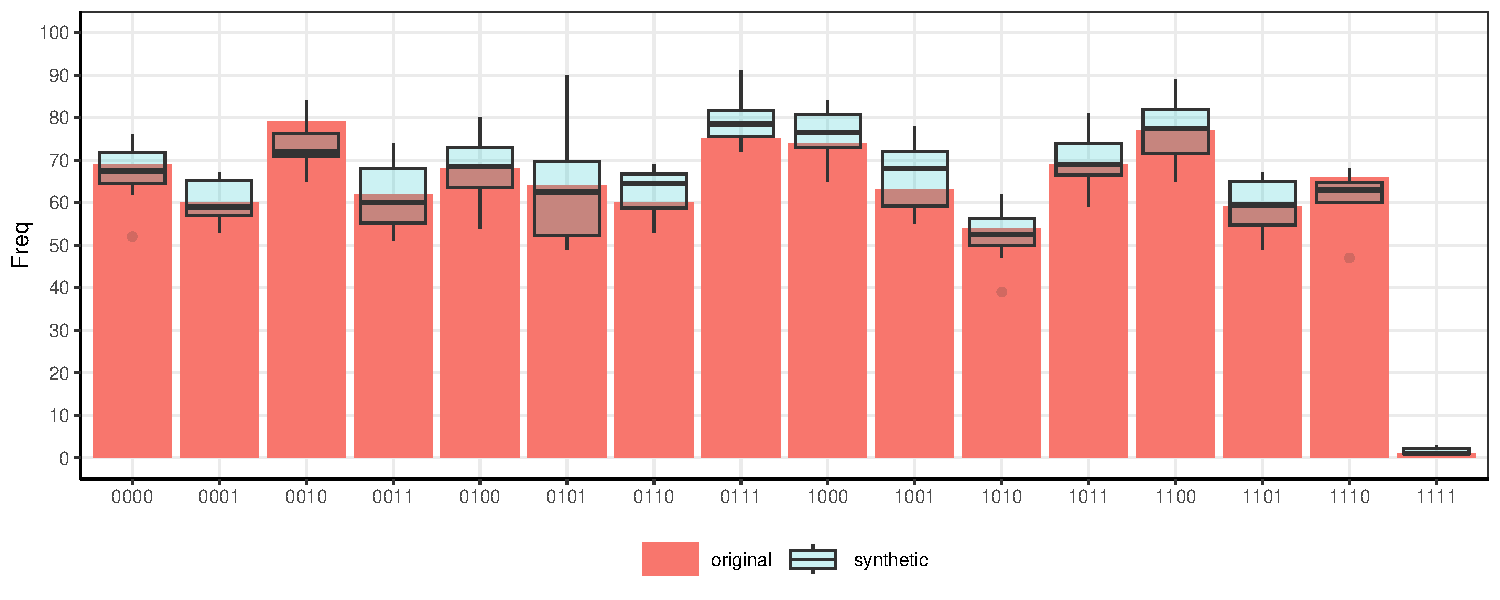
\includegraphics[width=\textwidth]{../graphs/graph_cart_histogram_compare_10.pdf}
    \label{fig:cart_histogram_compare_10}
\end{figure}

\section{The attack}

In this section, we describe an attack scenario.  The basic idea is that an attack is a game between two entities.  On one side, there is a statistical agency who has the data and wants to release it in a privacy preserving way.  On the other side, there is an attacker who wants to identify someone in the data (either membership or attribute inference). The question is what can the attacker learn from a released synthetic data set about an individual they do not have knowledge of?

In this scenario, we assume a `strong' attacker similar to the attack model in differential privacy (DP).  In so doing, we assume that the attacker knows the SDG used to generate the synthetic data.  In our case, this is sequential CART.  They know all observations except the last one.  Further, given the nature of the data, they know all 16 possible combinations that the last record could be.  In this attack, the attacker sees the synthetic data and then runs the same CART-based SDG for each of the 16 different possibilities, sequentially.  Then, they update their beliefs about what the last record could be.

Figure \ref{fig:attacker_default} illustrates the results of this attack with each attack using 10 synthetic data sets.  In the top left cell, the attacker guesses that the last record in the original data is 0,0,0,0.  They then generate 10 synthetic data sets using a CART-based SDG and compare the histogram to the released synthetic data, as shown in figure \ref{fig:compare}.  Remember, the released synthetic data replicates the single unique record found in the original data (1,1,1,1).  

\begin{figure}[!h]
    \centering
    \caption{Histogram of 16 worlds x 10 synthetic datasets}
    \resizebox{\textwidth}{!}{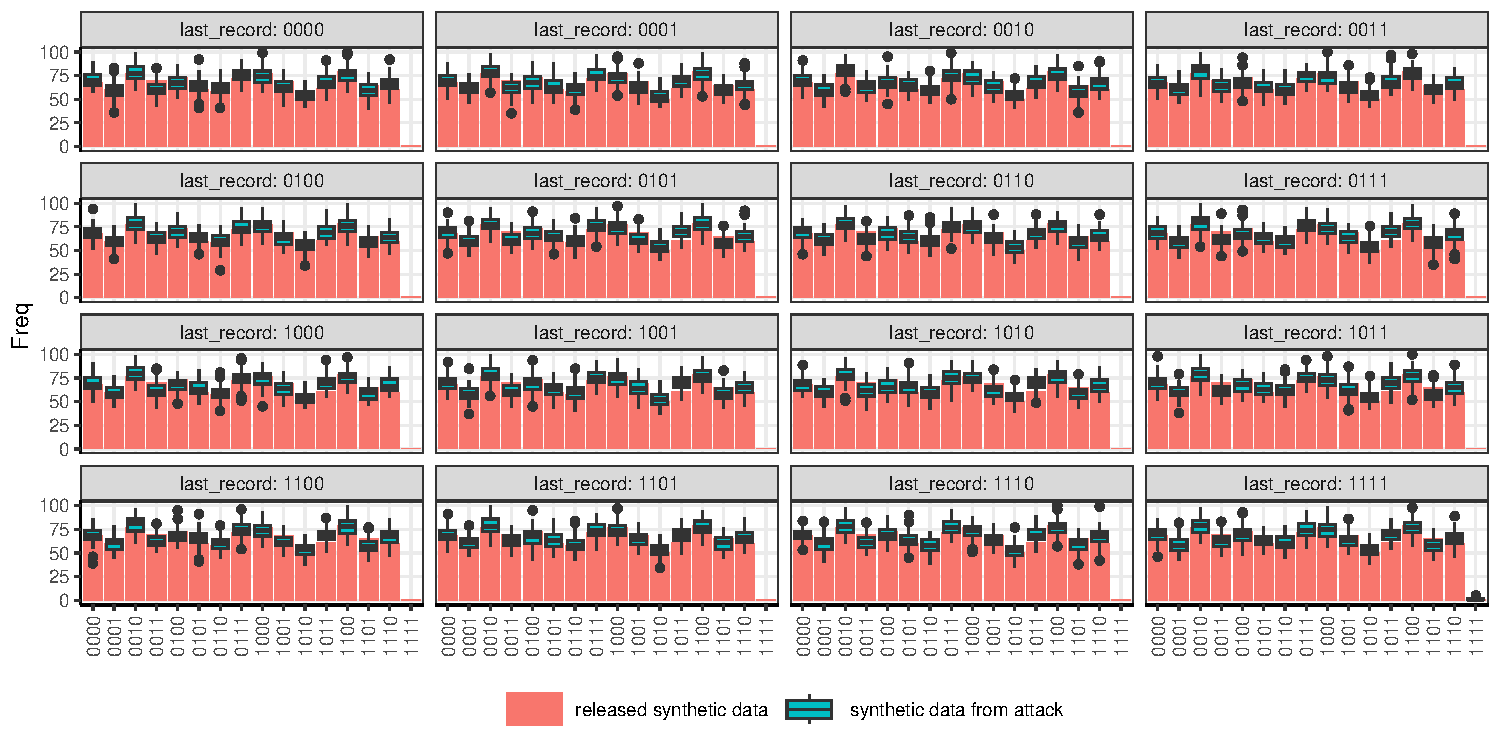
\includegraphics{../graphs/graph_attacker_default.pdf}}
    \label{fig:attacker_default}
\end{figure}

If the attacker guesses that the last record is 0,0,0,0, then they are not able to replicate the single unique record in the synthetic data.  As stated earlier, the reason is that a record may not be in the synthetic data if it is in the original data, but it can only be in the synthetic data if it is also in the original data. 

Next, they update their beliefs about the last record and guess that the last record in the original data is 0,0,0,1.  They then repeat the process as described above.  This is shown in the top row, second column from the left.  Like their first guess, they cannot replicate the released synthetic data.  

The attacker then repeats this process for all 16 possible combinations of the last record.  Finally, if they guess that the last record is 1,1,1,1, then they are able to replicate the released synthetic data, as shown in the bottom, right cell.  The result is a successful attack with confirmation that guess about the values of the last, unique observation is correct.

\section{Disclosure risk measures}

Our results show that CART can produce synthetic data that is disclosive because it replicates unique records from the original data set without adding sufficient noise.  By itself, this is not a problem.  However, this is a problem if we are not able to measure this disclosure.  The literature on privacy measures for synthetic data is well-developed \cite{wagner2018technical}.  One reason why there are so many measures of privacy is because there is no one agreed upon understanding of either what defines risk nor how one should measure it.  

We use three commonly understood measures of privacy implemented by the Synthpop package in R \cite{raab2024practical}: identity risk, uniques, and attribute risk.  In table \ref{table:disclosure_risk_1}, the columns display these three risk measures in the original and synthetic data (the rows).  For reference, we replicated table \ref{table:disclosure_risk_1} with 10 synthetic copies from figure \ref{fig:cart_histogram_compare_10}, as shown in table \ref{table:disclosure_risk_10} in the Appendix.  Results are qualitatively similar.  

\begin{table}[]
    \centering
    \caption{Disclosure risk measures}
    % latex table generated in R 4.4.0 by xtable 1.8-4 package
% Tue Jan 14 12:47:47 2025
\begin{tabular}{lrr}
  \toprule
data & identity & attribute \\ 
  \midrule
Original & 0.00 & 0.00 \\ 
  Synthetic & 0.00 & 0.00 \\ 
   \bottomrule
\end{tabular}

    \label{table:disclosure_risk_1}
\end{table}

In the first column, we display the identity disclosure risk for the original and synthetic data, as shown in the first and second row, respectively.  This measures the ability to identify individuals in the data from a set of known characteristics, i.e. `keys'. The maximum number of keys are one less than the total number of variables in the data.  Here, the keys are the first 3 binary variables ($q$), but this choice is arbitrary as all variables are binary.  Specifically, it measures the percent of all records in the data for which the keys identify a unique record in the synthetic data ($UiS$) and in the original data ($UiO$).  

The identity risk measures are 0 for both the original and synthetic data.  The measure is correct because we know that there are multiple combinations of $var1=(0,1)$, $var2=(0,1)$, $var3=(0,1)$.  In our data, there is zero risk of identity disclosure because there is no unique combination of observations with keys that number three or less variables.

In the second column, we display the unique records for the original and synthetic data.  This measures records in the dataset that are unique and thus more vulnerable to re-identification, particularly when matched with external data sources.  There is one record that is unique in both the original and synthetic data.  Therefore, the measure correctly captures the unique record in both data sets.

The fact that the synthetic data replicates the unique record is a red flag and should be considered to be a problem to be solved by the owner of the original data who wishes to release a privacy protected synthetic copy.  One possible option could be to produce another synthetic data set with a different seed.  A second idea is to release multiple synthetic data sets.  However, neither solves the problem.  As described earlier, even if one released 10 synthetic data sets, as shown in figure \ref{fig:cart_histogram_compare_10}, one might solve the specific problem of replicated uniques as observations of the disclosive record in synthetic data would range from 0 to 3, but this would not solve the problem of disclosure from an attack.  

There are two ways to protect the unique observation in the original data.  One is to not reproduce the unique observation in the synthetic data.  The second is to protect the unique observation by adding sufficient noise such that the frequency of 1,1,1,1 in the synthetic data were similar to the frequency of other combination of the four variables.  

In the third column, we display the attribute disclosure risk.  Attribute disclosure refers to the ability to identify a previously unknown characteristic of an individual.  In this approach, an attacker who wants to infer a sensitive attribute ($t$), has access to synthetic data, and knows one or more identifiers in the original data ($q$, i.e. composite keys, as in above).  Attribute risk is a subset of the proportion of records in the original for which the keys ($q$) in the synthetic data is disclosive. $q$ is disclosive if all records in the synthetic data with the same $q$ have a constant target ($t$), i.e. no variation in $t$.  According to this measure, there is 0 risk of attribute disclosure in the original or synthetic data.  This is a not correct because we know that when $q=111$, there is a unique record if $t=1$.  

How can it be that there is no attribute disclosure risk when we know there is an attribute disclosure risk?  The answer is that there is only an attribute disclosure risk when $t$ is constant.  In other words, when there is no variation within $q$.  As a result, there is only an attribute disclosure risk when there are 0 copies of the unique record in the synthetic data.  We can see this if we examine the frequency table from 10 synthetic data copies \ref{table:frequency_10_data_sets}, as shown in figure \ref{fig:cart_histogram_compare_10}.  If there is at least 1 unique record, then there is no attribute risk because there are 2 values of $t=(0,1)$ within $q$, but there is an attribute disclosure risk if a synthetic data set is released without a unique record.  This is a problem because the measure incorrectly estimates risk.

In summary, none of the risk measures examined here indicate that there is a problem with disclosure risk in our data.  Unique records is the only risk measure that does indicate there is a problem, but this is an accident of the seed.  If we used another seed, with less than or greater than 1 unique record in the synthetic data, then this measure would not indicate a problem.  Therefore, the main issue of concern is that we know there is a disclosure problem (because we created it), but the disclosure risk measures commonly used in the literature do not capture the problem.  

\section{Increasing privacy}

The good news.  We can correct the problem of disclosure risk in synthetic data generated from CART-based SDGs.  If we modify the parameters to prevent overfitting, then the disclosure problem goes away.  Multiple options exist to do this.  We use two: increase the minimum number of observations per terminal node to 75 (default is 5) and increase the complexity parameter to 0.05 (default is 1e$^{-8}$), as shown in figure \ref{fig:compare_modified}.  We arrived at these values after doing sensitivity tests, as shown in figure \ref{fig:compare_modified_sensitivity}.  While values below these do not add enough noise to the data to reduce disclosure risks, these adjustments can reduce disclosure risks.

\begin{figure}[!h]
    \centering
    \caption{Compare original and synthetic data}
    \begin{subfigure}{0.48\textwidth}
        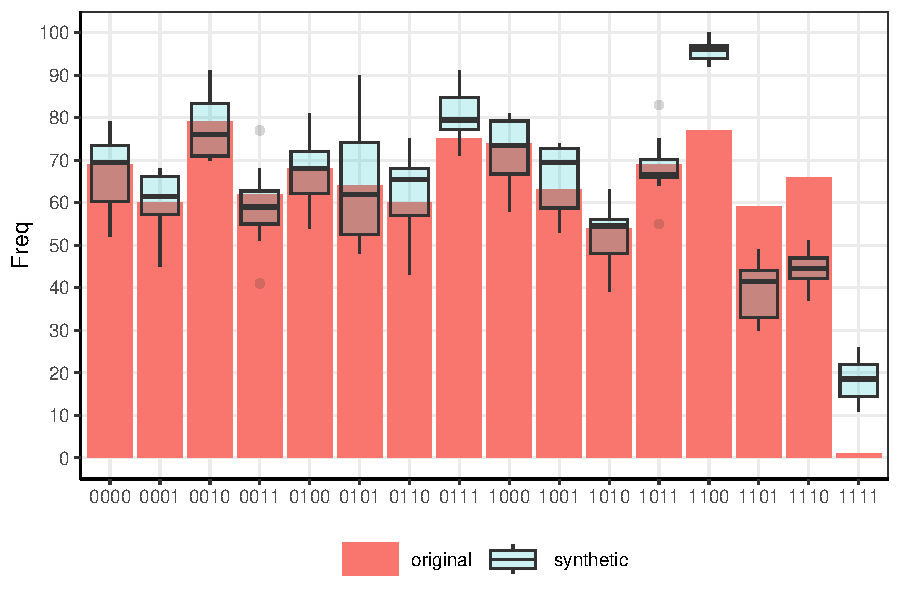
\includegraphics[width=\textwidth]{../graphs/graph_cart_modified_mb_histogram_compare_10.pdf}
        \caption{Minimum bucket is 75}
        \label{fig:attacker_modified_mb}
    \end{subfigure}
    \hfill
    \begin{subfigure}{0.48\textwidth}
        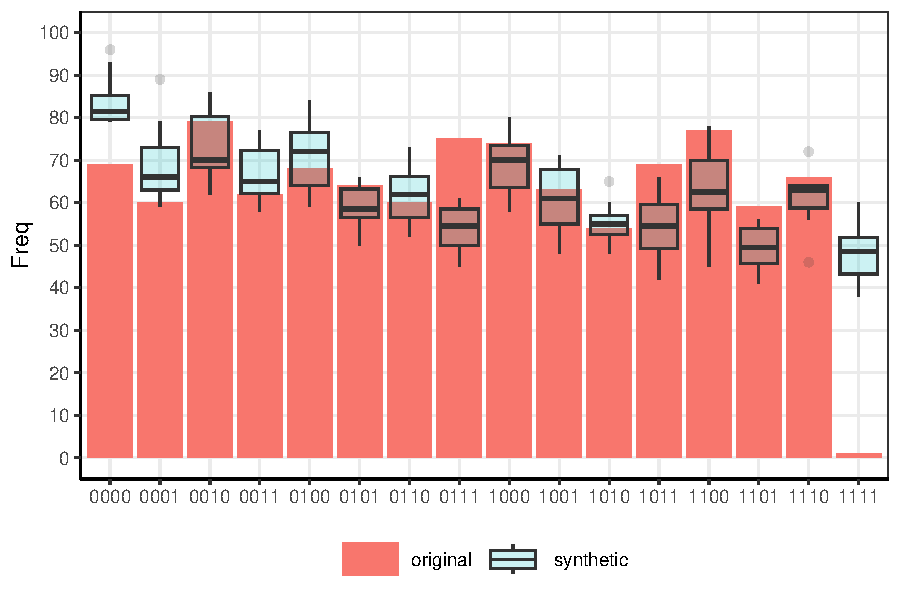
\includegraphics[width=\textwidth]{../graphs/graph_cart_modified_cp_histogram_compare_10.pdf}
        \caption{Complexity parameter is 0.05}
        \label{fig:attacker_modified_cp}
    \end{subfigure}
    \label{fig:compare_modified}
\end{figure}

The bad news.  First, the modified synthetic data may increase privacy, but the sacrifice is lower utility.  Even with 10 synthetic data sets, figure \ref{fig:compare_modified} is less representative of the original data set than \ref{fig:cart_histogram_compare_10}.  Second, in an important way, we are choosing to decrease utility in order to increase privacy.  Remember, as we have shown, no commonly used disclosure risk measure indicates that there is a problem.  In a real world example, this would raise the question of whether such sacrifices are justified when risks are not apparent.

\section{Discussion}


4.1 The Utility-Privacy Trade-Off

Our findings confirm the long-held understanding of a utility-privacy trade-off in synthetic data generation. CART models, despite their perceived robustness, are not immune to this trade-off.

4.2 Limitations of Current Privacy Metrics

The inability of common metrics to capture disclosure risks highlights the need for enhanced evaluation tools. Relying on these metrics alone may result in an underestimation of privacy vulnerabilities.

4.3 Implications for Practice

The results emphasize the need for cautious use of CART-based SDGs, particularly when handling datasets with unique records. Practitioners should consider:

    •   Implementing robust parameter tuning to mitigate risks.
    •   Combining CART with other privacy-preserving techniques.
    •   Developing new metrics to capture nuanced risks.

\section{Conclusion}

This study demonstrates that CART-based SDGs are susceptible to privacy risks, particularly in scenarios involving unique records. While parameter adjustments can enhance privacy, they necessitate a reduction in utility. Importantly, common privacy metrics failed to detect these risks, underscoring the limitations of existing tools.

Key Takeaways

    1.  CART-based models are not inherently immune to the utility-privacy trade-off.
    2.  Common privacy metrics may fail to detect significant risks.
    3.  Sacrificing utility is often necessary, but only if risks are known in advance.


\begin{credits}
\subsubsection{\ackname} This work was supported by a grant from the German Federal Ministry of Education and Research (grant number 16KISA096) with funding from the European Union—NextGenerationEU.  Reproducible files are located here: \url{https://github.com/jonlatner/KEM\_GAN/tree/main/latner/projects/simulation}

\subsubsection{\discintname}
The authors have no competing interests to declare that are relevant to the content of this article.
\end{credits}


%%%%%%%%%%%%%%%%%%%%%%%%%%%%%%%%
% Bibliography
%%%%%%%%%%%%%%%%%%%%%%%%%%%%%%%%
\bibliographystyle{splncs04}
\bibliography{references}

%%%%%%%%%%%%%%%%%%%%%%%%%%%%%%%%
% Appendix
%%%%%%%%%%%%%%%%%%%%%%%%%%%%%%%%
\clearpage
\appendix
\section{Appendix}\label{appendix}
\setcounter{figure}{0}    
\setcounter{table}{0}    
\renewcommand*\thetable{\Alph{section}.\arabic{table}}
\renewcommand*\thefigure{\Alph{section}.\arabic{figure}}
\renewcommand{\theHfigure}{\Alph{section}.\arabic{table}}
\renewcommand{\theHtable}{\Alph{section}.\arabic{figure}}

\begin{table}[]
    \centering
    \caption{Disclosure risk measures}
    % latex table generated in R 4.5.0 by xtable 1.8-4 package
% Wed Aug 13 15:48:18 2025
\begin{tabular}{lrr}
  \toprule
Data & Identity Risk ($repU$) & Attribute Risk ($DiSCO$) \\ 
  \midrule
Original & 0.00 & 0.00 \\ 
  Synthetic 1 & 0.00 & 0.00 \\ 
  Synthetic 2 & 0.00 & 6.60 \\ 
  Synthetic 3 & 0.00 & 0.00 \\ 
  Synthetic 4 & 0.00 & 0.00 \\ 
  Synthetic 5 & 0.00 & 0.00 \\ 
  Synthetic 6 & 0.00 & 0.00 \\ 
  Synthetic 7 & 0.00 & 0.00 \\ 
  Synthetic 8 & 0.00 & 6.60 \\ 
  Synthetic 9 & 0.00 & 0.00 \\ 
  Synthetic 10 & 0.00 & 0.00 \\ 
  Average & 0.00 & 1.32 \\ 
   \bottomrule
\end{tabular}

    \label{table:disclosure_risk_10}
\end{table}


\begin{table}[h!]
    \centering
    \caption{Attribute risk measures from 10 synthetic data sets}
    \rowcolors{1}{white}{lightgray}
    % latex table generated in R 4.4.0 by xtable 1.8-4 package
% Thu Dec 19 16:23:49 2024
\begin{tabular}{lrrrr}
  \toprule
m & Dsyn & iS & DiS & DiSCO \\ 
  \midrule
1 & 0 & 100 & 0 & 0 \\ 
  2 & 6.8 & 100 & 6.7 & 6.6 \\ 
  3 & 0 & 100 & 0 & 0 \\ 
  4 & 0 & 100 & 0 & 0 \\ 
  5 & 0 & 100 & 0 & 0 \\ 
  6 & 0 & 100 & 0 & 0 \\ 
  7 & 0 & 100 & 0 & 0 \\ 
  8 & 6.2 & 100 & 6.7 & 6.6 \\ 
  9 & 0 & 100 & 0 & 0 \\ 
  10 & 0 & 100 & 0 & 0 \\ 
  Average & 1.3 & 100 & 1.34 & 1.32 \\ 
   \bottomrule
\end{tabular}

    \label{table:attribute_risk_10}
\end{table}

\begin{table}[]
    \centering
    \caption{Frequency statistics for original and synthetic data}
    \rowcolors{1}{white}{lightgray}
    % \resizebox{.95\textwidth}{!}{% latex table generated in R 4.4.0 by xtable 1.8-4 package
% Mon Dec 16 16:27:40 2024
\begin{tabular}{lrrrrrrrrrrr}
  \toprule
   & \multicolumn{1}{l}{Original} & \multicolumn{10}{c}{Synthetic Data} \\ \cmidrule(lr){3-12}
 Combine & 0 & 1 & 2 & 3 & 4 & 5 & 6 & 7 & 8 & 9 & 10 \\ 
 \midrule
0000 & 69 & 68 & 66 & 71 & 73 & 76 & 62 & 72 & 52 & 64 & 67 \\ 
  0001 & 60 & 60 & 53 & 57 & 56 & 58 & 60 & 67 & 67 & 57 & 67 \\ 
  0010 & 79 & 77 & 71 & 73 & 71 & 71 & 84 & 65 & 70 & 77 & 74 \\ 
  0011 & 62 & 70 & 51 & 56 & 68 & 63 & 55 & 74 & 57 & 68 & 52 \\ 
  0100 & 68 & 73 & 63 & 80 & 54 & 61 & 79 & 65 & 73 & 66 & 71 \\ 
  0101 & 64 & 60 & 77 & 49 & 66 & 52 & 90 & 52 & 53 & 65 & 71 \\ 
  0110 & 60 & 58 & 68 & 66 & 61 & 69 & 56 & 67 & 65 & 64 & 53 \\ 
  0111 & 75 & 72 & 91 & 86 & 81 & 80 & 77 & 82 & 77 & 75 & 72 \\ 
  1000 & 74 & 77 & 84 & 80 & 73 & 70 & 81 & 82 & 65 & 76 & 73 \\ 
  1001 & 63 & 69 & 66 & 57 & 68 & 73 & 56 & 68 & 75 & 78 & 55 \\ 
  1010 & 54 & 50 & 54 & 57 & 51 & 47 & 50 & 39 & 62 & 58 & 54 \\ 
  1011 & 69 & 61 & 59 & 77 & 71 & 66 & 69 & 75 & 69 & 68 & 81 \\ 
  1100 & 77 & 79 & 77 & 76 & 83 & 78 & 66 & 65 & 88 & 70 & 89 \\ 
  1101 & 59 & 65 & 52 & 54 & 57 & 66 & 67 & 59 & 65 & 49 & 60 \\ 
  1110 & 66 & 60 & 68 & 60 & 64 & 68 & 47 & 65 & 62 & 64 & 60 \\ 
  1111 & 1 & 1 & 0 & 1 & 3 & 2 & 1 & 3 & 0 & 1 & 1 \\ 
   \bottomrule
\end{tabular}
}
    % latex table generated in R 4.4.0 by xtable 1.8-4 package
% Mon Dec 16 16:27:40 2024
\begin{tabular}{lrrrrrrrrrrr}
  \toprule
   & \multicolumn{1}{l}{Original} & \multicolumn{10}{c}{Synthetic Data} \\ \cmidrule(lr){3-12}
 Combine & 0 & 1 & 2 & 3 & 4 & 5 & 6 & 7 & 8 & 9 & 10 \\ 
 \midrule
0000 & 69 & 68 & 66 & 71 & 73 & 76 & 62 & 72 & 52 & 64 & 67 \\ 
  0001 & 60 & 60 & 53 & 57 & 56 & 58 & 60 & 67 & 67 & 57 & 67 \\ 
  0010 & 79 & 77 & 71 & 73 & 71 & 71 & 84 & 65 & 70 & 77 & 74 \\ 
  0011 & 62 & 70 & 51 & 56 & 68 & 63 & 55 & 74 & 57 & 68 & 52 \\ 
  0100 & 68 & 73 & 63 & 80 & 54 & 61 & 79 & 65 & 73 & 66 & 71 \\ 
  0101 & 64 & 60 & 77 & 49 & 66 & 52 & 90 & 52 & 53 & 65 & 71 \\ 
  0110 & 60 & 58 & 68 & 66 & 61 & 69 & 56 & 67 & 65 & 64 & 53 \\ 
  0111 & 75 & 72 & 91 & 86 & 81 & 80 & 77 & 82 & 77 & 75 & 72 \\ 
  1000 & 74 & 77 & 84 & 80 & 73 & 70 & 81 & 82 & 65 & 76 & 73 \\ 
  1001 & 63 & 69 & 66 & 57 & 68 & 73 & 56 & 68 & 75 & 78 & 55 \\ 
  1010 & 54 & 50 & 54 & 57 & 51 & 47 & 50 & 39 & 62 & 58 & 54 \\ 
  1011 & 69 & 61 & 59 & 77 & 71 & 66 & 69 & 75 & 69 & 68 & 81 \\ 
  1100 & 77 & 79 & 77 & 76 & 83 & 78 & 66 & 65 & 88 & 70 & 89 \\ 
  1101 & 59 & 65 & 52 & 54 & 57 & 66 & 67 & 59 & 65 & 49 & 60 \\ 
  1110 & 66 & 60 & 68 & 60 & 64 & 68 & 47 & 65 & 62 & 64 & 60 \\ 
  1111 & 1 & 1 & 0 & 1 & 3 & 2 & 1 & 3 & 0 & 1 & 1 \\ 
   \bottomrule
\end{tabular}

    \label{table:frequency_10_data_sets}
\end{table}


\begin{figure}[!h]
    \centering
    \caption{Compare original and synthetic data}
    \begin{subfigure}{0.9\textwidth}
        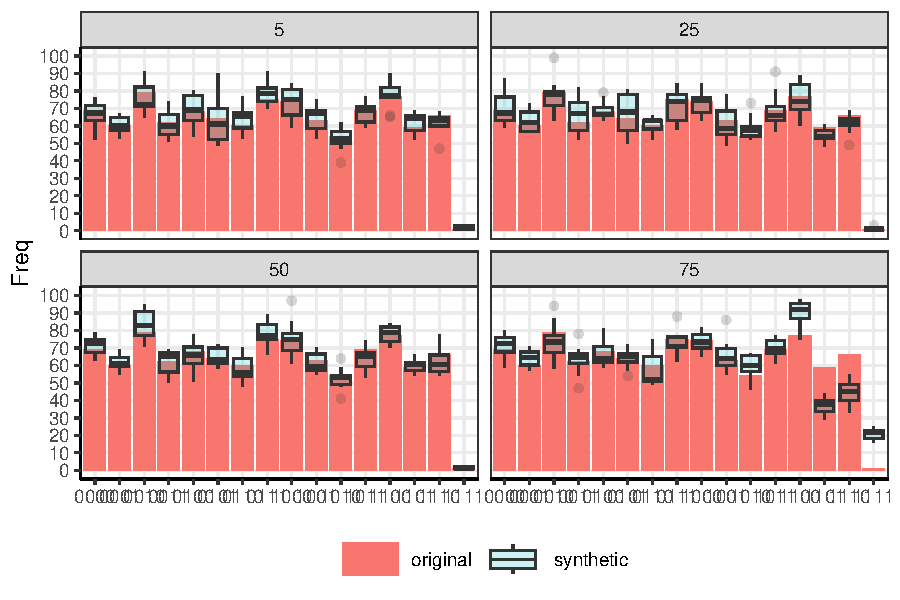
\includegraphics[width=\textwidth]{../graphs/graph_cart_modified_mb_histogram_compare_10_v2.pdf}
        \caption{Minimum bucket (default is 5)}
        \label{fig:attacker_modified_mb_sensitivity}
    \end{subfigure}
    \hfill
    \begin{subfigure}{0.9\textwidth}
        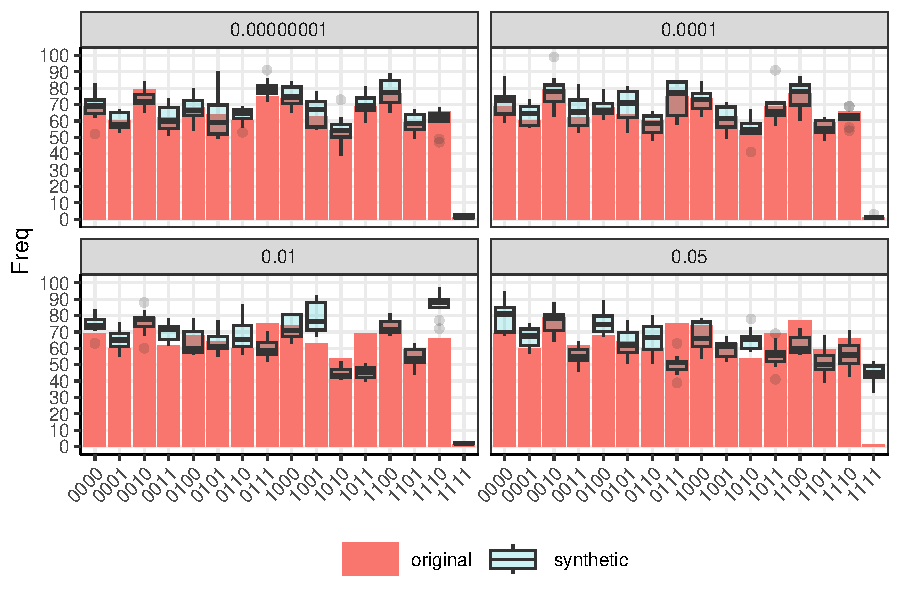
\includegraphics[width=\textwidth]{../graphs/graph_cart_modified_cp_histogram_compare_10_v2.pdf}
        \caption{Complexity parameter (default is 10$^{-8}$)}
        \label{fig:attacker_modified_cp_sensitivity}
    \end{subfigure}
    \label{fig:compare_modified_sensitivity}
\end{figure}


\begin{figure}[!h]
    \centering
    \caption{Datasynthesizer with DP}
    \resizebox{\textwidth}{!}{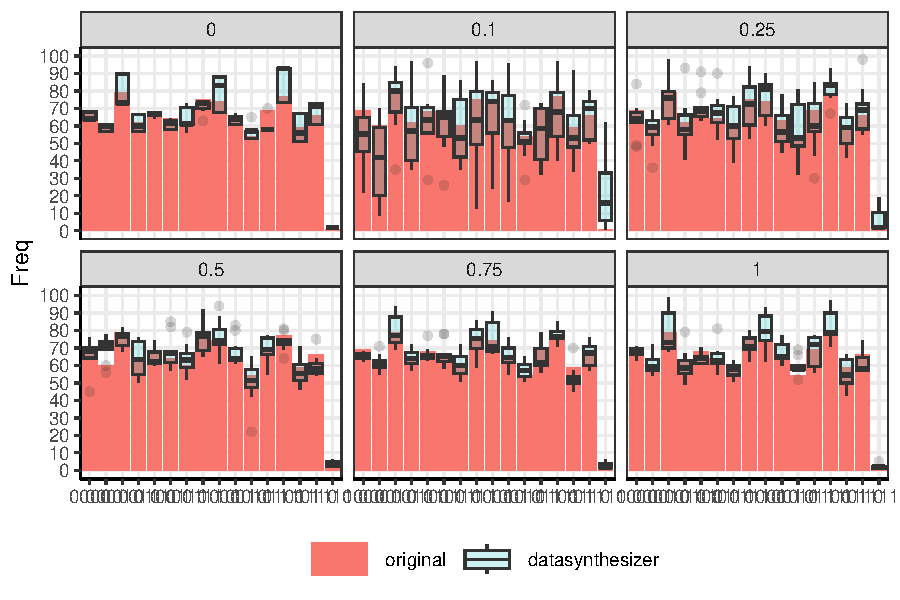
\includegraphics{../graphs/graph_dp_datasynthesizer_compare_histogram_10.pdf}}
    \label{fig:dp_datasynthesizer}
\end{figure}

\clearpage
\begin{table}[h!]
    \caption{SD2011}
    \label{tab:attribute_risk_sd2011}

    \begin{subtable}[t]{\textwidth} % 45% of the main table width
        \centering
        \caption{Original}
        \rowcolors{1}{white}{lightgray}
        % latex table generated in R 4.4.0 by xtable 1.8-4 package
% Sat Dec 21 09:14:34 2024
\begin{tabular}{lrrrr}
  \toprule
m & Dsyn & iS & DiS & DiSCO \\ 
  \midrule
1 & 45.2 & 64.84 & 33.36 & 8.96 \\ 
  2 & 46.18 & 65.48 & 33.68 & 9.9 \\ 
  3 & 46.98 & 65.34 & 33.96 & 10.46 \\ 
  4 & 46.6 & 64.32 & 33.06 & 9.68 \\ 
  5 & 45.26 & 64.32 & 32.98 & 8.88 \\ 
  Average & 46.044 & 64.86 & 33.408 & 9.576 \\ 
   \bottomrule
\end{tabular}

    \end{subtable}
    \hspace{0.05\textwidth} % Horizontal space between subtables

    \begin{subtable}[t]{\textwidth} % Another 45% of the main table width
        \centering
        \caption{Modified (depress = 1)}
        \rowcolors{1}{white}{lightgray}
        % latex table generated in R 4.4.0 by xtable 1.8-4 package
% Thu Dec 19 11:53:25 2024
\begin{tabular}{lrrrr}
  \toprule
m & Dsyn & iS & DiS & DiSCO \\ 
  \midrule
1 & 100 & 64.84 & 64.84 & 5.74 \\ 
  2 & 100 & 64.02 & 64.02 & 5.78 \\ 
  3 & 100 & 64.72 & 64.72 & 6.04 \\ 
  4 & 100 & 63.72 & 63.72 & 5.42 \\ 
  5 & 100 & 64.88 & 64.88 & 5.84 \\ 
  Average & 100 & 64.436 & 64.436 & 5.764 \\ 
   \bottomrule
\end{tabular}

    \end{subtable}
\raggedleft{Attribute disclosure measures for depress from keys: sex age region placesize}
\end{table}

\end{document}
